

\transition{Abstração -- Espaços de endereçamento}{mem:addressspace}

\begin{frame}{\insertlecture}
	É o conjunto de endereços de memória interna/principal
	que um processo pode usar.
	Cada processo tem seu próprio espaço independente
	do espaço usado por outros processo, com algumas
	exceções.
	
	Normalmente o gerenciamento do endereçamento \'e
	feito pelo sistema operacional.	
	\pause\\
	Estes espaços normalmente são gerenciados utilizando duas
	técnicas clássicas de alocação de memória:
	\begin{itemize}
		\item Troca de memória ({\em swapping});
		\item Memória virtual.
	\end{itemize}	
\end{frame}


\begin{frame}{Espaço de endereçamento do processo}

\begin{columns}

\begin{column}{0.45\textwidth}

%%% Local Variables: 
%%% mode: latex
%%% TeX-master: t
%%% End: 

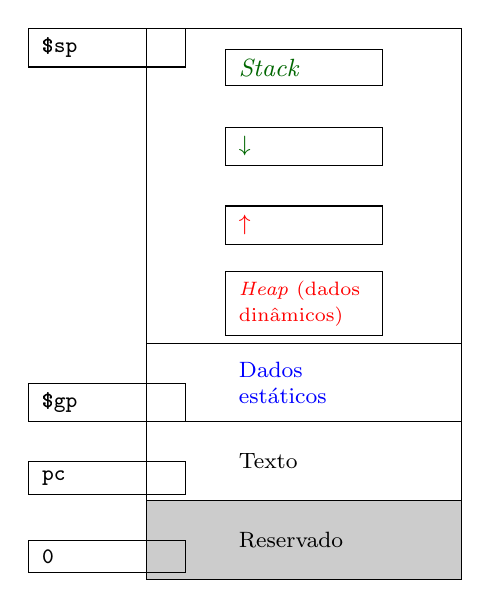
\begin{tikzpicture}
  \node[rectangle,draw,minimum width=4cm,minimum
  height=1cm,fill=gray!40]  (reserved) {Reservado};
  \node[rectangle,draw,minimum width=4cm,minimum
  height=1cm] (text) [above of=reserved] {Texto};
  \node[rectangle,draw,minimum width=4cm,minimum
  height=1cm] (static) [above of=text] {\color{blue}Dados estáticos};
  \node (heap) [above of=static] {\scriptsize \color{red}{\em Heap} (dados
    dinâmicos)};
  \node (up) [above of=heap] {\color{red}$\uparrow$};
  \node (down) [above of=up] {\color{green!40!black}$\downarrow$};
  \node (stack) [above of=down] {\small {\color{green!40!black}\em Stack}};
  \node[rectangle,draw,minimum width=4cm,minimum height=6cm,yshift=5mm] (rect) [above of=static] {};

  \node [left of=reserved,xshift=-15mm,anchor=north] {\tt 0};
  \node [left of=text,xshift=-15mm,anchor=north] {\tt pc};
  \node [left of=static,xshift=-15mm,anchor=north] {\tt \$gp};
  \node [left of=stack,xshift=-15mm,anchor=south] {\tt \$sp};

\end{tikzpicture}
\end{column}

\small
\begin{column}{0.55\textwidth}
\only<1>{
\begin{tabbing}
stru\= ct S \{\\
	\>float c;\\
	\>float d;\\
\}\\
main() \{\\
	\>{\color{blue}static int a};\\
	\>{\color{green!30!black} int b};\\
	\>struct S *s;\\

	\>{\color{red}s = (struct S*)(malloc(sizeof(struct S)))};\\
\}\\
\end{tabbing}
}

\only<2>{
\begin{itemize}
	\item Seção de texto (código executável);
	\item Seção de dados contendo variáveis 
	globais inicializadas;
	\item Mapeamento das variáveis globais não
	inicializadas;
	\item Texto, dados, das bibliotecas compartilhadas,
	\item Mapeamento de memória de arquivos abertos;
	\item Segmentos de memória compartilhadas;
	\item Mapeamentos anônimos de memória, por exemplo,
		pelo uso de {\tt malloc()}.
\end{itemize}
}
\end{column}
\end{columns}

\end{frame}

\transition{Troca de mem\'oria -- {\em swapping}}{mem:swap}

\begin{frame}{\insertlecture}

\begin{columns}

\begin{column}{.4\textwidth}

\begin{center}
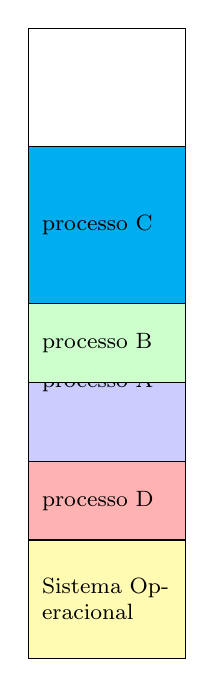
\begin{tikzpicture}
	\tikzset{every node/.style={minimum width=2cm,text width=1.65cm,font=\footnotesize,anchor=south,draw}}
	\node[minimum height=1.5cm,fill=yellow!30] (so) at (0,0) {Sistema Operacional};
	\node[minimum height=8cm] (so) at (0,0) {};	
	\node<1-3>[minimum height=2cm,fill=blue!20] (so) at (0,1.5cm) {processo A};
	\node<7>[minimum height=2cm,fill=blue!20] (so) at (0,2.5cm) {processo A};
	\node<2-5>[minimum height=1cm,fill=green!20] (so) at (0,3.5cm) {processo B};
	\node<3-7>[minimum height=2cm,fill=cyan] (so) at (0,4.5cm) {processo C};
	\node<5-7>[minimum height=1cm,fill=red!30] (so) at (0,1.5cm) {processo D};
\end{tikzpicture}	
\end{center}

\end{column}
	
\begin{column}{.6\textwidth}
	\small
	\only<1->{(1) Somente {\color{blue!40!black}Processo A} na memória\\}
	\only<2->{(2) {\color{green!40!black}Processo B} criado ou trazido do disco\\}
	\only<3->{(3) {\color{blue}Processo C} criado ou trazido do disco\\}
	\only<4->{(4) {{\color{blue!40!black}Processo A} \'e retirado \\}}
	\only<5->{(5) {\color{red}Processo D} criado ou trazido do disco}
	\only<6->{(6) {\color{green!40!black}Processo B} é retirado\\}
	\only<7->{(7) {\color{blue!40!black}Processo A} retorna para a 
				memória, porém em uma localização (endereço) diferente\\}
\end{column}	
	
\end{columns}	
	
\end{frame}

\begin{frame}{Exerc\'icios}

\begin{enumerate}
	\item Verificar a utilizaç\~ao da mem\'oria {\em swap}
	usando o comando {\tt top};
	\item Verificar a alocaç\~ao de segmentos de um 
		programa qualquer utilizando os comandos:
		\begin{itemize}
			\item {\tt cat /proc/<pid>/maps}
			\item {\tt pmap <pid>} 
		\end{itemize}
\end{enumerate}

\end{frame}

\def\thetitle{Gerenciamento da memória livre}
\subsubsection{\thetitle}

\begin{frame}{\thetitle}
	
	\begin{itemize}
		\item Mapa de bits
		\item Lista encadeada\\ algoritmos de alocaç\~ao:
			\begin{itemize}
				\item first fit: primeiro encaixe;
				\item next fit: ''memoriza'' primeiro
					encaixe com mem\'oria suficiente;
				\item best fit: encaixa no segmento de tamanho
				mais pr\'oximo do requerido;
				\item worst fit: aloca no maior segmento
					de mem\'oria dispon\'ivel.					
			\end{itemize}
	\end{itemize}

\end{frame}

\begin{frame}{Exercício}
	\small
	Considere um sistema de troca de processos
	entre a memória e o disco no qual a memória
	é composta pelos seguintes tamanhos de segmentos:
	10KB, 4KB, 20KB, 18KB, 7KB, 9KB, 12KB e 15KB. 
	Qual seguimento 
	é preenchido pela solicitação de espaço de:
	\begin{enumerate}
	\item 12KB,
	\item 10KB,
	\item 9KB,
	\end{enumerate}
	para os algoritmos de preenchimento
	 {\em first fit, best fit, worst fit, next fit.}	
\end{frame}
